\documentclass{beamer}

\usepackage[utf8]{inputenc}
\usepackage{tikz}

\usetikzlibrary{arrows,positioning,fit,shapes}



\usetheme{Verona}

\title{Operational Semantics for VMs in Hafnium}
\institute{Aarhus University}
\date{\today}
\author[Liu, Stepanenko, Trieu, Birkedal]
{\underline{Z.~Liu}, S.~Stepanenko, A.~Trieu, L.~Birkedal}

\institute[Aarhus]
{
  Department of Computer Science\\
  Aarhus University
}

% notations
\newcommand*{\defined}{\triangleq}
\newcommand*{\maps}{\rightarrow}
\newcommand*{\derived}{::=}

% definitions
\newcommand*{\CONF}{\text{ExecConf}}
\newcommand*{\STATE}{\text{State}}
\newcommand*{\MEM}{\text{GlobalMem}}
\newcommand*{\SSS}{\text{ShareStates}}
\newcommand*{\PID}{\text{PID}}
\newcommand*{\PT}{\text{PageTable}}
\newcommand*{\AS}{\text{AccessState}}
\newcommand*{\OS}{\text{OwnershipState}}
\newcommand*{\REGS}{\text{Registers}}
\newcommand*{\ADDR}{\text{Address}}
\newcommand*{\WORD}{\text{Word}}
\newcommand*{\VMID}{\text{VMID}}
\newcommand*{\REGNAMES}{\text{RegisterName}}
\newcommand*{\MODE}{\text{ExecMode}}
\newcommand*{\DONE}{\text{DoneState}}
\newcommand*{\INSTR}{\text{Instruction}}
\newcommand*{\MB}{\text{MailBox}}

% parameters
\newcommand*{\PABITS}{\text{ADDR\_BITS}}
\newcommand*{\PPBITS}{\text{PAGE\_BITS}}
\newcommand*{\PPIDBITS}{\text{PID\_BITS}}
\newcommand*{\PAMAX}{\text{ADDR\_MAX}}
\newcommand*{\PPMAX}{\text{PAGE\_MAX}}
\newcommand*{\PPIDMAX}{\text{PID\_MAX}}
\newcommand*{\PWBITS}{\text{WORD\_BITS}}
\newcommand*{\PWMAX}{\text{WORD\_MAX}}
\newcommand*{\PVMMAX}{\text{VM\_MAX}}


% instructions
\newcommand*{\instrm}[1]{\mathtt{#1}}
\newcommand*{\instr}[1]{\texttt{#1}}

% expressions
\newcommand*{\EI}[1]{\mathtt{ExecInstr} \; {#1}}
\newcommand*{\RP}[1]{\mathtt{Repeat} \; {#1}}
\newcommand*{\DN}[1]{\mathtt{Done} \; {#1}}
\newcommand*{\NXT}[1]{\mathtt{Next} \; {#1}}

% functions
\newcommand*{\decode}{\text{decode}}
\newcommand*{\pid}{\text{pid}}
\newcommand*{\addr}{\text{addr}}

% SOME/NONE
\newcommand{\SOME}{\mathtt{Some}}
\newcommand{\NONE}{\mathtt{None}}

% TRUE/FALSE
\newcommand{\TRUE}{\mathtt{True}}
\newcommand{\FALSE}{\mathtt{False}}


\begin{document}

\frame{\titlepage}



\begin{frame}
  \frametitle{Settings of Hafnium}
  \begin{figure}
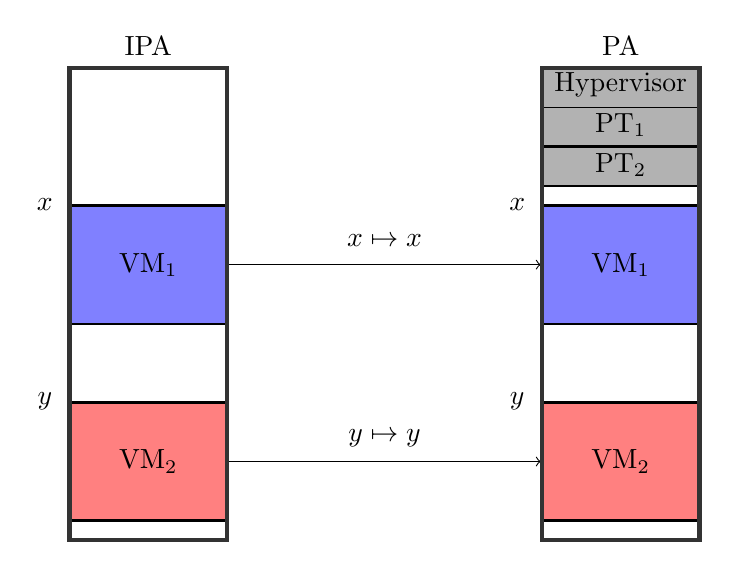
\begin{tikzpicture}[node distance=1cm, on grid]
 \tikzset{
pagetable/.style = {draw, minimum width=2cm,text height = 0.20cm},
memory/.style= {rectangle , draw = black, thick, minimum width = 2cm},
address space/.style = { rectangle, draw=black!80, ultra thick,minimum width=2cm,minimum height=6cm}}

\pgfdeclarelayer{foreground}
\pgfsetlayers{main,foreground}

    \begin{pgfonlayer}{foreground}
      \node [address space] (IPA)  at (-3,0) {};
      \node [address space] (PA) at (3,0) {};
      \node [above] at (PA.north) {PA};
      \node [above] at (IPA.north) {IPA};
    \end{pgfonlayer}
    \node [memory] (IP1)[fill = blue!50,minimum height = 1.5cm] at (-3,0.5) {VM$_{1}$};
    \node (X)[xshift = -3mm] at (IP1.north west) {$x$};
    \node [memory] (IP2)[fill = red!50,minimum height = 1.5cm] at (-3,-2) {VM$_{2}$};
    \node (Y)[xshift = -3mm] at (IP2.north west) {$y$};
    \node [memory] (PH)[fill = black!30,minimum height = 1.5cm] at (3,2.25) {};

    \node [pagetable] (PT1) at (3,2.25){PT$_{1}$};
    \node [pagetable] (PT2) at (3,1.75){PT$_{2}$};
    \node [above] at (PT1.north) {Hypervisor};

    \node [memory] (P1)[fill = blue!50,minimum height = 1.5cm] at (3,0.5) {VM$_{1}$}edge[<-] (IP1.east |- P1.west);
    \node (X')[xshift = -3mm] at (P1.north west) {$x$};
    \node [memory] (P2)[fill = red!50,minimum height = 1.5cm] at (3,-2) {VM$_{2}$}edge[<-] (IP2.east |- P2.west);
    \node (Y')[xshift = -3mm] at (P2.north west) {$y$};
    \node (E1)[minimum height = 0.5cm] at (0,0.8) {$x \mapsto x$};%edge[<-] (PT1.west);
    \node (E2)[minimum height = 0.5cm] at (0,-1.7) {$y \mapsto y$};%edge[<-] (PT2.west);

  \end{tikzpicture}

\caption{Stage-2 Memory Translation}
\end{figure}
\end{frame}

\begin{frame}
  \frametitle{Settings of Hafnium}
  \begin{itemize}
    \item Simple translation regime, 1-to-1 mapping at stage 2
    \item Fixed number of VMs, loaded at boot time
    \item One primary+mutiple secondary, the scheduler resides in the primary
    \item Sequential world, only one physical CPU
    \item FF-A framework is deployed for intercommunication between VMs
    \item TLB, cache, I/O etc. are ommited
  \end{itemize}
\end{frame}

\begin{frame}
  \frametitle{FF-A framework}
  \begin{itemize}
    \item Implemented as synchronous exceptions by Hafnium (at EL2)
    \item \texttt{hvc} calling conventions
      \begin{itemize}
        \item parameter registers: \texttt{W0}-\texttt{W7}
          \item return registers: \texttt{W0}-\texttt{W3}
          \end{itemize}
    \item CPU cycle management
      \begin{itemize}
        \item FFA\_RUN - can only be invoked by the primary VM
        \item FFA\_YIELD - can be invoked by secondary VMs
        \item FFA\_MSG\_WAIT - TODO
      \end{itemize}

  \end{itemize}
\end{frame}


\begin{frame}
  \frametitle{FF-A framework}
  Message passing(indirect messaging)
  \begin{itemize}
    \item RX page and TX page
    \item FFA\_MSG\_SEND - TODO
    \item FFA\_MSG\_POLL - TODO
  \end{itemize}
        \begin{figure}
        \caption{TODO - hypervisor copy...}
      \end{figure}
\end{frame}

\begin{frame}
  \frametitle{FF-A framework}
  Memory management
  \begin{itemize}
    \item All about ownership and access...
    \item Donation
    \item Sharing
      \item Lending
  \end{itemize}
  \begin{figure}
        \caption{TODO:ownership and access}
      \end{figure}
    \end{frame}

\begin{frame}
  \frametitle{FF-A framework}
  Memory management
  \begin{itemize}
    \item Three steps for one completed transaction
    \item Transaction descriptor, transfered via RX\&TX
  \end{itemize}
  \begin{figure}
        \caption{TODO:layout of descriptor}
      \end{figure}
       \begin{figure}
        \caption{TODO:three steps}
      \end{figure}
\end{frame}

\begin{frame}
  \frametitle{Execution Configuration}
\begin{figure}
  \begin{align*}
    \Phi &\in \CONF &\defined &\text{States} \times \MEM \times \SSS \\
    \delta s &\in \text{States} &\defined &\text{list(States)} \\
    \delta &\in \STATE &\defined &\PT \times \REGS \times \MB \\
    pt & \in \PT & \defined & \PID \maps (\OS \times \AS) \\
    mb & \in \MB &\defined &\text{TXPage} \times  \text{RXPage}\\
    tx & \in \text{TXPage} &\defined &\PID\\
    rx & \in \text{RXPage} &\defined &\PID \times \text{Bool} \times \WORD \times \VMID \\
    pid & \in \PID &\defined  &[ 0, \PPIDMAX ] \\
     v,n & \in \VMID &\defined  &[ 0, \PVMMAX ] \\
      & \;\;\;\; \OS & \derived & O | !O  ~~~~~~~  \AS  \derived  NA | EA | SA
  \end{align*}
  \caption{Execution Configuration: VM States.}
\end{figure}

\end{frame}

\begin{frame}
  \frametitle{Execution Configuration}
\begin{figure}
  \begin{align*}
      rs & \in \REGS &\defined  &\REGNAMES \maps \WORD \\
    rn & \in \REGNAMES &\defined &\text{SysRegs} \cup \text{GenRegs}\\
    mm & \in \MEM &\defined  &\ADDR \maps \WORD \\
    a & \in \ADDR &\defined  &[ 0, \PAMAX ] \\
    w & \in \WORD &\defined  &[ 0, \PWMAX ] \\
    sss & \in \SSS &\defined  &\WORD \maps \text{ShareState} \\
    ss & \in \text{ShareState} &\defined &\VMID \times \WORD \times \WORD \times (\VMID \times \PID +\\
                                           &&&\mathbb{N} \times \text{list}(\VMID \times \PID)) \times \text{FunctionID}\\
      & \;\;\;\; \text{SysRegs} &\derived & \mathtt{NV} | \mathtt{CNT\_VAL} | \mathtt{CNT\_CTL} | \dots \\
         & \;\;\;\; \text{GenRegs} &\derived & \mathtt{pc} | \mathtt {R0} | \mathtt{R1} | \dots
  \end{align*}
  \caption{Execution Configuration: Global Memory and Share States.}
\end{figure}

\end{frame}


\begin{frame}
  \frametitle{Syntax and Instructions}
\begin{figure}
  \begin{align*}
    \mu &\in \MODE &\derived & \mathtt{ExecInstr} \; v | \mathtt{Repeat} \; \mu | \mathtt{Done} \; \theta \\
    \theta &\in \DONE &\derived & \NXT{v} | \mathtt{Halt} | \mathtt{Fail}\\
    \\
    instr & \in  \INSTR &\derived & \instrm{br} \; r |\instrm{bne} \; r \; r |
                                    \instrm{mov} \; r \; w | \instrm{ldr} \; r\; r|
                                    \instrm{str} \; r \; r | \instrm{add} \; r \; r \; r \\
        & & & | \instrm{sub} \; r \; r \; r | \instrm{cmp} \; r \; r | \instrm{fail} | \instrm{halt} | \instrm{hvc} |\instrm{mrs} \; r\;r | \instrm{msr} \; r \; r\\
    fid & \in \text{FunctionID} &\derived & \tt{RUN} ~|~\tt{YIELD} ~|~\tt{MSG\_WAIT} ~|~\tt{MSG\_SEND}
                                            ~|~\tt{MSG\_POLL}~ \\
        &&&|~\tt{MEM\_DONATE}~|~\tt{MEM\_RETRIEVE\_REQ} ~|~ \tt{SUCC} ~|~\tt{ERROR}\\
        &&&|~\tt{MEM\_RETRIEVE\_RESP}~|~\tt{MEM\_SHARE} ~|~ \tt{MEM\_LEND}\\
        &&&|~\tt{MEM\_RECLAIM}~|~\tt{MEM\_RELINQUISH}\\
    err & \in \text{ErrorCode} &\derived & \tt{INV\_PARA} ~|~\tt{DENIED} ~|~\tt{BUSY}~|~\tt{RETRY}
  \end{align*}
  \caption{Syntax and Machine Instructions}
\end{figure}

\end{frame}

\begin{frame}
  \frametitle{Rules(Selected)}
 TODO
\end{frame}

\begin{frame}
  \frametitle{Rules(Selected)}
 TODO
\end{frame}



\end{document}
